\section*{Đề kiểm tra Chương 1}
\subsection*{Đề số 1}
\setcounter{ex}{0}\setcounter{bt}{0}
\Opensolutionfile{ans}[ans/ans-KT-101]
\noindent\textbf{I. PHẦN TRẮC NGHIỆM}
%[Phan Quốc Trí, Bai Giảng T10(2022)]%
\begin{ex}%[Phan Quốc Trí, Bai Giảng T10(2022)]%[0D1Y1-1]
	Trong các câu sau, câu nào không phải là mệnh đề?
	\choice
	{Hình bình hành có bốn cạnh bằng nhau}
	{\True Chúc bạn may mắn}
	{Số $8$ là số chính phương}
	{Cà Mau là tên một tỉnh của nước Việt Nam}
	\loigiai{
		Mệnh đề là một câu khẳng định \textbf{đúng} hoặc một câu khẳng định \textbf{sai}.
	}
\end{ex}
\begin{ex}%[Phan Quốc Trí, Bai Giảng T10(2022)]%[0D1Y1-1]
	Trong các câu sau, câu nào là mệnh đề?
	\choice
	{$x^2+x=2$}
	{Hôm nay trời đẹp quá!}
	{$2n+1$ chia hết cho 3}
	{\True Số 15 là một số nguyên tố}
	\loigiai{
\begin{itemize}
	\item $x^2+x=2$  là một khẳng định, nhưng không là mệnh đề. 
	\item  Hôm nay trời đẹp quá! không phải là mệnh đề.
	\item Câu $2n+1$ chia hết cho 3 là một khẳng định, nhưng không là mệnh đề. 
	\item  Số 15 là một số nguyên tố là một mệnh đề sai.
\end{itemize}
	}
\end{ex}
\begin{ex}%[Phan Quốc Trí, Bai Giảng T10(2022)]%[0D1Y1-2]
	Trong các mệnh đề sau, mệnh đề nào là mệnh đề \textbf{sai}?
	\choice
	{\True $\sqrt{3}$ là số nguyên}
	{$6$ chia hết cho $2$}
	{$5$ chia hết cho $5$}
	{$30$ là một số chẵn}
	\loigiai{
		Trong các mệnh đề đã cho, mệnh đề sai là \lq\lq$\sqrt{3}$ là số nguyên\rq\rq.
	}
\end{ex}
\begin{ex}%[Phan Quốc Trí, Bai Giảng T10(2022)]%[0D1Y1-2]
	Cho mệnh đề chứa biến $P(x): 3x+5\le x^2$ với $x$ là số thực. Mệnh đề nào sau đây là đúng?
	\choice
	{$P(3)$}
	{$P(4)$}
	{$P(1)$}
	{\True $P(5)$}
	\loigiai{
		$P(3)= 3.3+5\leqslant 3^2 \Leftrightarrow 14\leqslant 9$ là mệnh đề sai.\\
		$P(4) =3.4+5\leqslant 4^2 \Leftrightarrow 17\leqslant 16$ là mệnh đề sai.\\
		$P(1)=3.1+5\leqslant 1^2 \Leftrightarrow 8\leqslant 1$ là mệnh đề sai.\\
		$P(5) =3.5+5\leqslant 5^2 \Leftrightarrow 20\leqslant 25$ là mệnh đề đúng.}
\end{ex}
\begin{ex}%[Phan Quốc Trí, Bai Giảng T10(2022)]%[0D1Y1-3]
	Cho mệnh đề $P\colon$ \lq\lq  $9$ là số chia hết cho $3$\rq\rq. Mệnh đề phủ định của mệnh đề $P$ là
	\choice
	{$\overline{P}\colon$\lq\lq  $9$ là ước của $3$\rq\rq}
	{$\overline{P}\colon$\lq\lq  $9$ là bội của $3$\rq\rq}
	{\True $\overline{P}\colon$ \lq\lq  $9$ là số không chia hết cho $3$\rq\rq}
	{$\overline{P}\colon$\lq\lq  $9$ là số lớn hơn $3$\rq\rq}
	\loigiai{Mệnh đề $P\colon$\lq\lq  $9$ là số chia hết cho $3$\rq\rq      có mệnh đề phủ định là $\overline{P}\colon$ \lq\lq  $9$ là số không chia hết cho $3$\rq\rq.}
\end{ex}
\begin{ex}%[Phan Quốc Trí, Bai Giảng T10(2022)]%[0D1Y1-3]
	Cho mệnh đề \lq\lq$\forall x\in \mathbb{R},\, x^2+1>0$\rq \rq. Mệnh đề phủ định của mệnh đề đã cho là
	\choice
	{\lq\lq$\forall x\in \mathbb{R},\, x^2+1\leq 0$\rq \rq}
	{\lq\lq$\forall x\in \mathbb{R},\, x^2+1<0$\rq \rq}
	{\True \lq\lq$\exists x\in \mathbb{R},\, x^2+1\leq 0$\rq \rq}
	{\lq\lq$\exists x\in \mathbb{R},\, x^2+1>0$\rq \rq}
	\loigiai{
		Mệnh đề phủ định của mệnh đề \lq\lq$\forall x\in \mathbb{R},\, x^2+1>0$\rq \rq\, là \lq\lq$\exists x\in \mathbb{R},\, x^2+1\leq 0$\rq \rq.}
\end{ex}
\begin{ex}%[Phan Quốc Trí, Bai Giảng T10(2022)]%[0D1Y1-4]
	Cho mệnh đề $P\colon$ ``Tam giác $ABC$ cân tại $A$'', mệnh đề $Q\colon$ ``$AB=AC$''. Phát biểu mệnh đề ``$P$ kéo theo $Q$'' là
	\choice
	{Nếu $AB=AC$ thì tam giác $ABC$ cân tại $A$}
	{\True Nếu tam giác $ABC$ cân tại $A$ thì $AB=AC$}
	{Tam giác $ABC$ cân tại $B$ là điều kiện cần và đủ để $AB=AC$}
	{Tam giác $ABC$ cân tại $A$ khi và chỉ khi $AB=AC$}
	\loigiai{
		Mệnh đề ``$P$ kéo theo $Q$'' là ``Nếu tam giác $ABC$ cân tại $A$ thì $AB=AC$''.
	}
\end{ex}
\begin{ex}%[Phan Quốc Trí, Bai Giảng T10(2022)]%[0D1Y1-4]
	Cho mệnh đề $P$: \lq\lq Nếu tam giác có hai đường trung tuyến bằng nhau thì đó là tam giác cân\rq\rq. Mệnh đề nào sau đây là mệnh đề đảo của $P$?
	\choice
	{Tam giác có hai đường trung tuyến bằng nhau thì nó là tam giác cân}
	{\True Nếu tam giác $ABC$ cân thì tam giác đó có hai đường trung tuyến bằng nhau }
	{Tam giác là tam giác cân khi và chỉ khi nó có hai đường trung tuyến bằng nhau}
	{Tam giác là tam giác cân nếu nó có hai đường trung tuyến bằng nhau}
	\loigiai{
Mệnh đề đảo là \lq \lq Nếu tam giác $ABC$ cân thì tam giác đó có hai đường trung tuyến bằng nhau.\rq \rq		
	}
\end{ex}
\begin{ex}%[Phan Quốc Trí, Bai Giảng T10(2022)]%[0D1Y1-5]
	Mệnh đề "Bình phương mọi số thực đều không âm" mô tả mệnh đề nào dưới đây?
	\choice
	{"$\forall n\in\mathbb{N}: n^2\geq 0$"}
	{"$\exists x\in\mathbb{R}:x^2\geq 0$"}
	{\True "$\forall x\in\mathbb{R}: x^2\geq 0$"}
	{"$\forall x\in\mathbb{R}:x^2>0$"}
	\loigiai{
	Mệnh đề trên được viết lại dạng: \lq \lq $\forall x\in\mathbb{R}: x^2\geq 0$\rq \rq	
	}
\end{ex}
\begin{ex}%[Phan Quốc Trí, Bai Giảng T10(2022)]%[0D1B1-5]
	Mệnh đề nào sau đây là đúng?
	\choice
	{$\forall n\in\mathbb{N}\colon n^2>n$}
	{$\forall x\in\mathbb{R}\colon x^2<2$}
	{$\forall x\in\mathbb{Z}\colon 2x>1$}
	{\True $\exists x\in\mathbb{R}\colon x^2>x$}
	\loigiai
	{
		\begin{itemize}
			\item Mệnh đề ``$\forall n\in\mathbb{N}\colon n^2>n$'' sai vì với $n=1$ thì $n^2=1=n$.
			\item Mệnh đề ``$\forall x\in\mathbb{R}\colon x^2<2$'' sai vì với $x=2$ thì $x^2=4>2$.
			\item Mệnh đề ``$\forall x\in\mathbb{Z}\colon 2x>1$'' sai vì với $x=0$ thì $2x=0<1$.
			\item Mệnh đề ``$\exists x\in\mathbb{R}\colon x^2>x$'' đúng vì với $x=2$ thì $x^2=4$ nên $x^2>x$.
		\end{itemize}
	}
\end{ex}
\begin{ex}%[Phan Quốc Trí, Bai Giảng T10(2022)]%[0D1Y2-1]
	Hãy liệt kê các phần tử của tập hợp $X = \left\{ x \in \mathbb{Z} | 2x^2-5x+3=0 \right\}$.
	\choice
	{$X = \left\{1;\dfrac{3}{2} \right\}$}
	{\True $X = \{ 1 \}$}
	{$X = \left\{ \dfrac{3}{2} \right\}$}
	{$X = \varnothing$}
	\loigiai{
		Ta có $2x^2-5x+3=0\Leftrightarrow \hoac{&x=1\in \mathbb{Z}\\&x=\dfrac{3}{2}\notin \mathbb{Z}}$.\\
		Vậy $X = \{ 1 \}$.		
	}
\end{ex}
\begin{ex}%[Phan Quốc Trí, Bai Giảng T10(2022)]%[0D1B2-1]
	Viết tập hợp $A=\lbrace x \in \mathbb{Z}|x^2<17 \rbrace $ theo cách liệt kê các phần tử, ta được tập hợp nào sau đây?
	\choice{\True $ \lbrace -4;-3;-2;-1;0;1;2;3;4 \rbrace $}
	{$ \lbrace 1;2;3;4 \rbrace $}
	{$\lbrace 0;1;2;3;4  \rbrace $}
	{$ \lbrace -4; -3;-2;-1 \rbrace $}
	\loigiai{Ta có $x^2<17\Leftrightarrow \left|x\right|<\sqrt{17}\Leftrightarrow -\sqrt{17}<x<\sqrt{17}$.\\
		Vì $x\in \mathbb{Z}$ nên $A=\lbrace -4;-3;-2;-1;0;1;2;3;4 \rbrace $.
	}
\end{ex}

\begin{ex}%[Phan Quốc Trí, Bai Giảng T10(2022)]%[0D1Y2-1]
	Cho tập hợp $A=\left\{ x \in \mathbb{N}| x^2+2x-3=0 \right\}$. Mệnh đề nào sau đây là đúng?
	\choice
	{\True $-3 \notin A$}
	{$A=\left\{1;-3\right\}$}
	{$1 \notin A$}
	{$A=\left\{1;3\right\}$}
	\loigiai{
		Ta có $x^2+2x-3=0 \Leftrightarrow \hoac{&x=1\\&x=-3}$. Do $x \in \mathbb{N}$ nên $A=\left\{1\right\}$. Do đó $-3 \notin A$.
	}
\end{ex}
\begin{ex}%[Phan Quốc Trí, Bai Giảng T10(2022)]%[0D1Y2-2]
	Cho tập $A=\{a;b;5\}$. Số tập con của tập $A$ là
	\choice
	{$5$}
	{\True $8$}
	{$7$}
	{$4$}
	\loigiai{Tập con của $A$ là $\varnothing, \{a\}, \{b\},\{5\}, \{a;b\}, \{a;5\}, \{b;5\}, \{a;b;5\} $. Vậy số tập con của $A$ là $8$.
	}
\end{ex}
\begin{ex}%[Phan Quốc Trí, Bai Giảng T10(2022)]%[0D1Y2-2]
	Có bao nhiêu tập $ X $ thỏa mãn $ \{a;b\} \subset X \subset \{1;2;a;b\}$?
	\choice
	{$3$}
	{$2$}
	{\True $4$}
	{$5$}
	\loigiai{
		Các tập $ X $ thỏa mãn là $ \{a;b\} $, $ \{1;a;b\} $, $ \{2;a;b\} $, $ \{1;2;a;b\} $.
	}
\end{ex}
\begin{ex}%[Phan Quốc Trí, Bai Giảng T10(2022)]%[0D1B4-1]
	Cho tập hợp $A=\{x\in\mathbb{R}|-3<x\le 3\}$. Mệnh đề nào dưới đây đúng?
	\choice
	{$A=\{-2;-1;0;1;2;3\}$}
	{\True $A=(-3;3]$}
	{$A=[-3;3]$}
	{$A=[-3;3)$}
	\loigiai{
		Từ giả thiết, có $A=(-3;3]$.
	}
\end{ex}
\begin{ex}%[Phan Quốc Trí, Bai Giảng T10(2022)]%[0D1B2-2]
	Cho tập hợp $A = \left\{x \in \mathbb{N}\big| x^2 + 8x + 15 = 0\right\}$. Khẳng định nào sau đây đúng?
	\choice
	{$A = \left\{-3;-5\right\}$}
	{\True $A =\varnothing$}
	{$A = \left\{\varnothing\right\}$}
	{$A = \left\{0\right\}$}
	\loigiai{
		Phương trình $x^2+8x+15=0$ có hai nghiệm $x_1=-3$, $x_2=-5$. Tuy nhiên $x_1, x_2\notin \mathbb{N}$. Vậy $A=\varnothing$.
	}
\end{ex}
\begin{ex}%[Phan Quốc Trí, Bai Giảng T10(2022)]%[0D1B2-2]
	Gọi $A$ là tập hợp tất cả các hình bình hành và $B$ là tập hợp tất cả các hình chữ nhật. Trong các kết luận sau, kết luận nào đúng?
	\choice
	{$A \subset B$}
	{\True $B \subset A$}
	{$A=B$}
	{$A \cap B=\varnothing$}
	\loigiai{
		Ta có hình chữ nhật là hình bình hành có một góc vuông nên $B \subset A$.
	}
\end{ex}

\begin{ex}%[Phan Quốc Trí, Bai Giảng T10(2022)]%[0D1Y2-2]
	Khẳng định nào sau đây là đúng?
	\choice
	{$ \mathbb{R}\subset\mathbb{Q} $}
	{$ \mathbb{Z}\subset\mathbb{N} $}
	{$ \mathbb{Q}\subset\mathbb{Z} $}
	{\True $ \mathbb{N}\subset\mathbb{R} $}
	\loigiai{
		Ta có $ \mathbb{N}\subset\mathbb{Z}\subset\mathbb{Q}\subset\mathbb{R} $.
	}
\end{ex}
\begin{ex}%[Phan Quốc Trí, Bai Giảng T10(2022)]%[0D1Y3-1]
	Cho hai tập hợp $X=\left\{1;3;5;8\right\}$ và $Y=\left\{3;5;7;9\right\}$. Tập hợp $X\cup Y$ bằng
	\choice
	{$\left\{1;7;9\right\}$}
	{$\left\{3;5\right\}$}
	{$\left\{1;3;5\right\}$}
	{\True $\left\{1;3;5;7;8;9\right\}$}
	\loigiai{
		Ta có $X\cup Y=\left\{1;3;5;7;8;9\right\}$.
	}
\end{ex}
\begin{ex}%[Phan Quốc Trí, Bai Giảng T10(2022)]%[0D1Y3-1]
	Cho $A=\{2;3;6;7\}, B=\{3;6;8\}$. Tập hợp $A\cap B$ bằng
	\choice
	{$\{3;6;8\}$}
	{$\{2;3;6;7;8\}$}
	{\True $\{3;6\}$}
	{$\{2;7\}$}
	\loigiai{
		Ta có $A\cap B=\{3;6\}.$
	}
\end{ex}
\begin{ex}%[Phan Quốc Trí, Bai Giảng T10(2022)]%[0D1Y3-2]
	Cho hai tập hợp $A=\{2;4;6;9\}$, $B=\{1;2;3;4\}$. Tập $A \setminus B$ bằng tập hợp nào sau đây?
	\choice
	{$\{2;4\}$}
	{$\{1;3\}$}
	{\True $\{6;9\}$}
	{$\{6;9;1;3\}$}
	\loigiai{
		Ta có: $A \setminus B=\{6;9\}$.}
\end{ex}

\begin{ex}%[Phan Quốc Trí, Bai Giảng T10(2022)]%[0D1Y3-2] 
	Cho tập $ X=\left\lbrace 0;1;2;3;4;5 \right\rbrace$ và tập $ A=\left\lbrace 0;2;4 \right\rbrace  $. Tìm phần bù của $ A $ trong $ X $.	
	\choice
	{$ \varnothing $}
	{$ \left\lbrace 2;4 \right\rbrace $ }
	{$ \left\lbrace 0;1;3 \right\rbrace  $}
	{\True $ \left\lbrace 1;3;5 \right\rbrace  $}
	\loigiai
	{
		Ta có phần bù của $ A $ trong $ X $ bằng tập $ X\setminus A=\left\lbrace 1;3;5 \right\rbrace  $.	
	}
\end{ex}
\begin{ex}%[Phan Quốc Trí, Bai Giảng T10(2022)]%[0D1B3-1]
	Cho hai tập hợp $A=(-3;3)$ và $B=(0;+\infty)$. Tìm  $A \cup B$.
	\choice
	{\True $ A \cup B = (-3;+\infty) $}
	{$ A \cup B = [-3;+\infty) $}
	{$ A \cup B = [-3;0) $}
	{$ A \cup B = (0;3) $}
	\loigiai{
		\immini{Tập hợp $A=(-3;3)$ có biểu diễn là}{ 
			\begin{tikzpicture}[scale=1, font=\footnotesize, line join = round, line cap = round, >=stealth]
				\draw[thick,->] (-2,0)node[below=6pt]{$-\infty$} -- (0,0) node[scale=1.5]{\bf ( } node[below=6pt]{$-3$} -- (3,0) node[scale=1.5]{\bf )} node[below=6pt]{$3$} -- (5,0)node[below=6pt]{$+\infty$};
				\foreach \i in {1,...,10} 
				\draw ($(0,0)-(.2*\i,0)$) node[scale=.6]{/};
				\draw ($(0,0)$) node[scale=.6]{/};
				\foreach \i in {1,...,9} 
				\draw ($(3,0)+(.2*\i,0)$) node[scale=.6]{/};
				\draw ($(3,0)$) node[scale=.6]{/};
		\end{tikzpicture}}
		\immini{Tập hợp $B=(0;+\infty)$ có biểu diễn là}{
			\begin{tikzpicture}[scale=1, font=\footnotesize, line join = round, line cap = round, >=stealth]
				\draw[thick,->] (-2,0)node[below=6pt]{$-\infty$}--(1,0) node[scale=1.5]{\bf (} node[below=6pt]{$0$}-- (5,0)node[below=6pt]{$+\infty$};
				\foreach \i in {1,...,15} 
				\draw ($(1,0)-(.2*\i,0)$) node[scale=.6,rotate=60]{/};
				\draw ($(1,0)$) node[scale=.6,rotate=60]{/};
				%	\foreach \i in {1,...,5} 
				%	\draw ($(4,0)+(.2*\i,0)$) node[scale=.6,rotate=60]{/};
		\end{tikzpicture}}
		\noindent Do đó $A \cup B=(-3;+\infty)$.
	}
\end{ex}
\begin{ex}%[Phan Quốc Trí, Bai Giảng T10(2022)]%[0D1B3-1]
	Cho tập hợp $X=(-\infty;2] \cap (-6;+\infty)$. Khẳng định nào sau đây là đúng?
	\choice
	{\True $X=(-6;2]$}
	{$(-6;+\infty)$}
	{$X=(-\infty;+\infty)$}
	{$X=(-\infty;2]$}
	\loigiai{
		Ta có: $X=(-\infty;2] \cap (-6;+\infty)=(-6;2]$.}
\end{ex}

\begin{ex}%[Phan Quốc Trí, Bai Giảng T10(2022)]%[0D1B3-2]
	Cho tập hợp $ A=[-2;3] $ và $ B=(1;5] $. Khi đó $ A\setminus B $ là
	\choice
	{$(-2;1]$}
	{$(-2;-1)$}
	{$[-2;1) $}
	{\True $[-2;1]$}
	\loigiai{
		Ta có $ A\setminus B =[-2;3]\setminus(1;5]= [-2;1]$. 
	}
\end{ex}

 \begin{ex}%[Phan Quốc Trí, Bai Giảng T10(2022)]%[0D1B3-2]
 	Cho tập hợp $A=\left\{x \in \mathbb{R} |  0 \le x+2 <5 \right\}$. Tập hợp $C_{\mathbb{R}}A$ bằng
 	\choice
 	{$(-\infty;-2)$}
 	{$(-\infty;-2] \cup (3;+\infty)$}
 	{\True $(-\infty;-2) \cup [3;+\infty)$}
 	{$[3;+\infty)$}
 	\loigiai{
 		Ta có: $C_{\mathbb{R}}A=(-\infty;-2) \cup [3;+\infty)$.}
 \end{ex}
\begin{ex}%[Phan Quốc Trí, Bai Giảng T10(2022)]%[0D1B3-3]
	Một lớp học có $25$ học sinh giỏi môn Toán, $23$ học sinh giỏi môn Lý, $14$ học sinh giỏi cả môn Toán và Lý và có $6$ học sinh không giỏi môn nào cả. Hỏi lớp đó có bao nhiêu học sinh?
	\choice
	{$26$}
	{$54$}
	{$68$}
	{\True $40$}
	\loigiai
	{
		Vì có $25$ học sinh giỏi môn Toán và $14$ học sinh giỏi cả môn Toán và Lý nên có $25-14=11$ học sinh chỉ giỏi môn Toán mà không giỏi môn Lý. \\
		Vì có $23$ học sinh giỏi môn Lý và $14$ học sinh giỏi cả môn Toán và Lý nên có $23-14=9$ học sinh chỉ giỏi môn Lý mà không giỏi môn Toán. \\
		Vậy lớp đó có $11+9+14+6=40$ học sinh.
	}
\end{ex}
\begin{ex}%[Phan Quốc Trí, Bai Giảng T10(2022)]%[0D1B3-3]
	Mỗi học sinh của lớp $10A$ đều chơi bóng đá hoặc bóng chuyền. Biết rằng có $25$ bạn chơi bóng đá, $20$ bạn chơi bóng chuyền và $10$ bạn chơi cả $2$ môn thể thao. Hỏi lớp $10A$ có bao nhiêu học sinh.
	\choice
	{$30$}
	{$55$}
	{$45$}
	{\True $35$}
	\loigiai{
		Ngoài sơ đồ Ven ta có thể dùng công thức số phần tử. Gọi $A$ là tập hợp các học sinh chơi bóng đá, $B$ là tập các học sinh chơi bóng chuyền. Do đó $A\cap B$ là tập các học sinh chơi cả hai môn. Ta có
		$$|A|=25, |B|=20, |A \cap B| =10.$$
		Số học sinh cả lớp là số phần tử của tập $A \cup B$. Theo công thức ta có $|A \cup B| = 25+20-10=35$ (học sinh).
	}
\end{ex}
\begin{ex}%[Phan Quốc Trí, Bai Giảng T10(2022)]%[0D1B3-1] 
	Cho các tập hợp $M=[-3;6]$ và $N=(-\infty; -2)\cup (3;+\infty)$. Khi đó $M\cap N$ là
	\choice
	{$(-\infty;-2)\cup (3;6)$}
	{$(-\infty;-2)\cup [3;+\infty)$}
	{\True $[-3;-2)\cup (3;6]$}
	{$(-3;-2)\cup (3;6)$}
	\loigiai{
		Biểu diễn trục số:  
		\begin{center}
			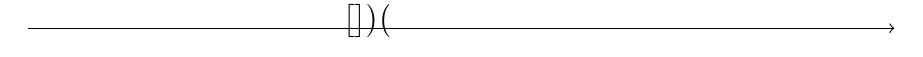
\begin{tikzpicture}
				\draw[->](-4,0)->(7,0);
				\IntervalLR{-4}{-3}
				\IntervalGR{}{}{\big[}{-3}
				\IntervalLR{6}{6.9}
				\IntervalGR{\big]}{6}{}{}
				\IntervalLR{-2}{3}
				\def\skipInterval{0.5cm}
				\IntervalGLF{\big)}{-2}{\big(}{3}
			\end{tikzpicture}
		\end{center}
		Từ hình vẽ, ta có
		Khi đó: $M\cap N= [-3;-2)\cup (3;6]$.}
\end{ex}

\begin{ex}%[Phan Quốc Trí, Bai Giảng T10(2022)]%%[Trần Ngọc Minh]%[301-320-Huỳnh Thanh Tiến]%[0D1B4-1]
	Tập hợp $(1;2)\cap\mathbb{N}$ là tập hợp nào sau đây?
	\choice
	{$\{1;2\}$}
	{$\{1\}$}
	{\True $\varnothing$}
	{$\{2\}$}
	\loigiai{
		Ta có $\mathbb{N}=\{0,1,2,\ldots\}$.
		Do đó 	$(1;2)\cap\mathbb{N}=\varnothing$.
	}
\end{ex}	
\begin{ex}%[Phan Quốc Trí, Bai Giảng T10(2022)]%[0D1B4-1]
	Cho $A=(-5;1]$, $B=[3;+\infty)$, $C=(-\infty;-2)$. Khẳng định nào sau đây đúng?
	\choice
	{$A\cap C=[-5;-2]$}
	{$A\cup B=(-5;+\infty)$}
	{$B\cup C=(-\infty;+\infty)$}
	{$\True B\cap C= \varnothing$}
	\loigiai{
		\begin{center}
			\begin{tikzpicture}
				\draw[->](-1,0)->(5,0);
				\IntervalLR{-1}{3}
				\def\skipInterval{0.5cm}
				\IntervalGRF{}{}{\big[}{3}
				\IntervalLR{4}{4.8}
				\def\skipInterval{0.5cm}
			\end{tikzpicture}\\
			\begin{tikzpicture}
				\draw[->](-1,0)->(5,0);
				\IntervalLR{-1}{1/2}
				\def\skipInterval{0.5cm}
				\IntervalLR{2}{4.9}
				\def\skipInterval{0.5cm}
				\IntervalGRF{\big)}{-2}{}{}
			\end{tikzpicture}
		\end{center}
		Từ biểu diễn tập nghiệm của $B$ và $C$ ta thấy $B\cap C= \varnothing$.
	}
\end{ex}
\begin{ex}%[Phan Quốc Trí, Bai Giảng T10(2022)]%%[0-HK2-2021, Trường THPT Trần Phú, Hải Phòng, năm học 2017 - 2018]%[Trần Quang Thạnh]%[0D1Y4-2]
	Cho tập hợp $A=[-2;3]$ và $B=(-2;5]$. Khi đó $A\setminus B$ là
	\choice
	{$[-2;5] $}
	{$(-2;-1) $}
	{$(3;5) $}
	{\True $\left\{-2\right\} $}
	\loigiai{
		Ta có $A\setminus B=\left\{-2\right\}$.
	}
\end{ex}
\begin{ex}%[Phan Quốc Trí, Bai Giảng T10(2022)]%[0D1B4-2]
	Cho các tập $A=\left\{x\in\mathbb{R}\mid x\ge -1\right\}$; $B=\left\{x\in\mathbb{R}\mid x<3\right\}$. Tập hợp $\mathbb{R}\setminus\left(A\cap B\right)$ là
	\choice
	{$[-1;3)$}
	{$(-\infty;-1]\cup(3;+\infty)$}
	{\True $(-\infty;-1)\cup[3;+\infty)$}
	{$(-1;3]$}
	\loigiai{
		Ta có $A\cap B=[-1;3)$, suy ra $\mathbb{R}\setminus\left(A\cap B\right)=(-\infty;-1)\cup[3;+\infty)$.
	}
\end{ex}
\begin{ex}%[Phan Quốc Trí, Bai Giảng T10(2022)]%[0D1K2-2]
	Tìm tất cả các giá trị của $m$ để đoạn $[m;m+3]$ là tập con của nửa khoảng $(-2;9]$.
	\choice
	{$-2\le m\le 6$}
	{$-2\le m<6$}
	{\True $-2<m\le 6$}
	{$-2<m<6$}
	\loigiai{
		Đoạn $[m;m+3]$ là tập con của nửa khoảng $(-2;9]$ khi và chỉ khi $\heva{& -2<m \\& m+3\le 9}\Leftrightarrow \heva{& -2<m \\& m\le 6}\Leftrightarrow -2<m\le 6.$
	}
\end{ex}



\noindent\textbf{II. PHẦN TỰ LUẬN}
\begin{bt}%[Phan Quốc Trí, Bai Giảng T10(2022)]%[0D1B4-1] 
	Cho $A=\left \{x \in \mathbb{R} \Big|  x \geq 3\right \}$ và $B=(-2 ; 7]$.  Tìm các tập hợp $A \cap B$, $A \cup B$.
	\loigiai{
		Ta có $A=\left \{x \in \mathbb{R} \Big|  x \geq 3\right \} = [3;+\infty )$. \\
		$A \cap B =[3;+\infty ) \cap (-2 ; 7] =    [3;7 ]$. \\
		$A \cup B = [3;+\infty ) \cup (-2 ; 7] = (-2;+\infty)$. 
	}
\end{bt}
\begin{bt}%[Phan Quốc Trí, Bai Giảng T10(2022)]%[0D1B3-2]
	Cho hai tập hợp $A=\left\{ 0;2 \right\}$ và $B=\left\{ 0;1;2;3;4 \right\}$. Tìm tất cả các tập hợp $X$ thỏa mãn $A\cup X=B$.
	\loigiai { 
		Vì $A\cup X=B$ nên $X$ chắc chắn có chứa các phần tử $1;3;4$\\
		Các tập $X$ có thể là $\left\{ 1;3;4 \right\},\,\left\{ 1;3;4;0 \right\},\,\left\{ 1;3;4;2 \right\},\,\left\{ 1;3;4;0;2 \right\}$}
\end{bt}
\begin{bt}%[Phan Quốc Trí, Bai Giảng T10(2022)]%[0D1K4-1]
	Cho hai tập hợp $A=(2m-1;m+3)$, $B=(-4;5)$. Tìm $m$ để
 $A\cap B=\varnothing $.
	\loigiai{
		Điều kiện: $2m-1<m+3 \Leftrightarrow m<4$.\\
	 Ta có  $A\cap B=\varnothing $ khi và chỉ khi $\left[
			\begin{aligned}
				&m+3\leqslant -4\\
				&2m-1\geqslant 5
			\end{aligned}\right. \Leftrightarrow \left[
			\begin{aligned}
				&m\leqslant -7\\
				&m\geqslant 3.
			\end{aligned}\right. $\\
			Đối chiếu điều kiện, ta được $m\leqslant -7$ hoặc $3\leqslant m<4$ thỏa yêu cầu bài toán.
	}
\end{bt}
\begin{bt}%[Phan Quốc Trí, Bai Giảng T10(2022)]%[0D1B3-3]
Lớp 10A có $45$ học sinh, trong đó có $18$ học sinh tham gia cuộc thi vẽ đồ họa trên máy tính, $24$ học sinh tham gia cuộc thi tin học văn phòng cấp trường và $9$ học sinh không tham gia cả hai cuộc thi này. Hỏi lớp 10A có bao nhiêu học sinh tham gia đồng thời cả hai cuộc thi?	
	\loigiai{
\immini{
Gọi $A$ là tập hợp các học sinh tham gia cuộc thi vẽ đồ họa trên máy tính. Suy ra $n(A)= 18$.\\
$B$ là tập hợp các học sinh tham gia  cuộc thi tin học văn phòng cấp trường. Suy ra $n(B)= 24$.\\
Ta có $A \cap B$ là tập hợp các học sinh tham gia đồng thời cả hai cuộc thi.\\
 $A \cup B$ là tập hợp các học sinh tham gia cuộc thi vẽ đồ họa trên máy tính hoặc tham gia  cuộc thi tin học văn phòng cấp trường. 
}{
	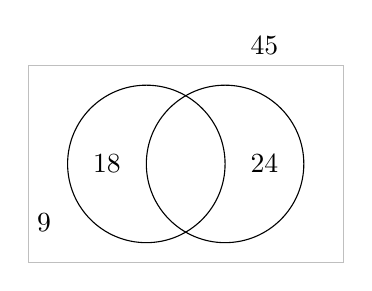
\begin{tikzpicture}
		\draw[] (0,0) circle ( 1.0cm);
		\draw (1.0,0) circle ( 1.0 cm);
		\draw (-0.5,0) node {$18$};
		\draw (1.5,0) node {$24$};
		\draw (-1.3,-0.75) node {$9$};
		\draw (1.5,1.5) node {$45$};
		\node[rectangle,
		draw = lightgray,
		minimum width = 4cm, 
		minimum height = 2.5cm] (r) at (0.5,0) {};
	\end{tikzpicture}
}
$$n \left(A \cup B \right)= 45-9=36.$$	
$$n \left( A \cap B \right) = n(A)+ n(B)-n(A \cup B)=18+24-36= 6.$$
Vậy có $6$  học sinh tham gia đồng thời cả hai cuộc thi.
	}
\end{bt}
\Closesolutionfile{ans}

\newpage
\begin{indapan}{10}
{ans/ans-KT-101}
\end{indapan}

\section*{Đề kiểm tra Chương 1}
\subsection*{Đề số 2}
\setcounter{ex}{0}\setcounter{bt}{0}
\Opensolutionfile{ans}[ans/ans-KT-102]
\noindent\textbf{I. PHẦN TRẮC NGHIỆM}
%[Thi thử, Sở GD và ĐT - Điện Biên, 2018]%[Dương BùiĐức, 12EX10]%[2D2Y3-2]
\begin{ex}%[Phan Quốc Trí, Bai Giảng T10(2022)]%[0D1Y1-1]
	Trong các câu sau, câu nào không phải là mệnh đề?
	\choice
	{Hình bình hành có bốn cạnh bằng nhau}
	{\True Chúc bạn may mắn}
	{Số $8$ là số chính phương}
	{Cà Mau là tên một tỉnh của nước Việt Nam}
	\loigiai{
		Mệnh đề là một câu khẳng định \textbf{đúng} hoặc một câu khẳng định \textbf{sai}.
	}
\end{ex}
\begin{ex}%[Phan Quốc Trí, Bai Giảng T10(2022)]%[0D1Y1-1]
	Trong các câu sau, câu nào là mệnh đề?
	\choice
	{$x^2+x=2$}
	{Hôm nay trời đẹp quá!}
	{$2n+1$ chia hết cho 3}
	{\True Số 15 là một số nguyên tố}
	\loigiai{
		\begin{itemize}
			\item $x^2+x=2$  là một khẳng định, nhưng không là mệnh đề. 
			\item  Hôm nay trời đẹp quá! không phải là mệnh đề.
			\item Câu $2n+1$ chia hết cho 3 là một khẳng định, nhưng không là mệnh đề. 
			\item  Số 15 là một số nguyên tố là một mệnh đề sai.
		\end{itemize}
	}
\end{ex}
\begin{ex}%[Phan Quốc Trí, Bai Giảng T10(2022)]%[0D1Y1-2]
	Trong các mệnh đề sau, mệnh đề nào là mệnh đề \textbf{sai}?
	\choice
	{\True $\sqrt{3}$ là số nguyên}
	{$6$ chia hết cho $2$}
	{$5$ chia hết cho $5$}
	{$30$ là một số chẵn}
	\loigiai{
		Trong các mệnh đề đã cho, mệnh đề sai là \lq\lq$\sqrt{3}$ là số nguyên\rq\rq.
	}
\end{ex}
\begin{ex}%[Phan Quốc Trí, Bai Giảng T10(2022)]%[0D1Y1-2]
	Cho mệnh đề chứa biến $P(x): 3x+5\le x^2$ với $x$ là số thực. Mệnh đề nào sau đây là đúng?
	\choice
	{$P(3)$}
	{$P(4)$}
	{$P(1)$}
	{\True $P(5)$}
	\loigiai{
		$P(3)= 3.3+5\leqslant 3^2 \Leftrightarrow 14\leqslant 9$ là mệnh đề sai.\\
		$P(4) =3.4+5\leqslant 4^2 \Leftrightarrow 17\leqslant 16$ là mệnh đề sai.\\
		$P(1)=3.1+5\leqslant 1^2 \Leftrightarrow 8\leqslant 1$ là mệnh đề sai.\\
		$P(5) =3.5+5\leqslant 5^2 \Leftrightarrow 20\leqslant 25$ là mệnh đề đúng.}
\end{ex}
\begin{ex}%[Phan Quốc Trí, Bai Giảng T10(2022)]%[0D1Y1-3]
	Cho mệnh đề $P\colon$ \lq\lq  $9$ là số chia hết cho $3$\rq\rq. Mệnh đề phủ định của mệnh đề $P$ là
	\choice
	{$\overline{P}\colon$\lq\lq  $9$ là ước của $3$\rq\rq}
	{$\overline{P}\colon$\lq\lq  $9$ là bội của $3$\rq\rq}
	{\True $\overline{P}\colon$ \lq\lq  $9$ là số không chia hết cho $3$\rq\rq}
	{$\overline{P}\colon$\lq\lq  $9$ là số lớn hơn $3$\rq\rq}
	\loigiai{Mệnh đề $P\colon$\lq\lq  $9$ là số chia hết cho $3$\rq\rq      có mệnh đề phủ định là $\overline{P}\colon$ \lq\lq  $9$ là số không chia hết cho $3$\rq\rq.}
\end{ex}
\begin{ex}%[Phan Quốc Trí, Bai Giảng T10(2022)]%[0D1Y1-3]
	Cho mệnh đề \lq\lq$\forall x\in \mathbb{R},\, x^2+1>0$\rq \rq. Mệnh đề phủ định của mệnh đề đã cho là
	\choice
	{\lq\lq$\forall x\in \mathbb{R},\, x^2+1\leq 0$\rq \rq}
	{\lq\lq$\forall x\in \mathbb{R},\, x^2+1<0$\rq \rq}
	{\True \lq\lq$\exists x\in \mathbb{R},\, x^2+1\leq 0$\rq \rq}
	{\lq\lq$\exists x\in \mathbb{R},\, x^2+1>0$\rq \rq}
	\loigiai{
		Mệnh đề phủ định của mệnh đề \lq\lq$\forall x\in \mathbb{R},\, x^2+1>0$\rq \rq\, là \lq\lq$\exists x\in \mathbb{R},\, x^2+1\leq 0$\rq \rq.}
\end{ex}
\begin{ex}%[Phan Quốc Trí, Bai Giảng T10(2022)]%[0D1Y1-4]
	Cho mệnh đề $P\colon$ ``Tam giác $ABC$ cân tại $A$'', mệnh đề $Q\colon$ ``$AB=AC$''. Phát biểu mệnh đề ``$P$ kéo theo $Q$'' là
	\choice
	{Nếu $AB=AC$ thì tam giác $ABC$ cân tại $A$}
	{\True Nếu tam giác $ABC$ cân tại $A$ thì $AB=AC$}
	{Tam giác $ABC$ cân tại $B$ là điều kiện cần và đủ để $AB=AC$}
	{Tam giác $ABC$ cân tại $A$ khi và chỉ khi $AB=AC$}
	\loigiai{
		Mệnh đề ``$P$ kéo theo $Q$'' là ``Nếu tam giác $ABC$ cân tại $A$ thì $AB=AC$''.
	}
\end{ex}
\begin{ex}%[Phan Quốc Trí, Bai Giảng T10(2022)]%[0D1Y1-4]
	Cho mệnh đề $P$: \lq\lq Nếu tam giác có hai đường trung tuyến bằng nhau thì đó là tam giác cân\rq\rq. Mệnh đề nào sau đây là mệnh đề đảo của $P$?
	\choice
	{Tam giác có hai đường trung tuyến bằng nhau thì nó là tam giác cân}
	{\True Nếu tam giác $ABC$ cân thì tam giác đó có hai đường trung tuyến bằng nhau }
	{Tam giác là tam giác cân khi và chỉ khi nó có hai đường trung tuyến bằng nhau}
	{Tam giác là tam giác cân nếu nó có hai đường trung tuyến bằng nhau}
	\loigiai{
		Mệnh đề đảo là \lq \lq Nếu tam giác $ABC$ cân thì tam giác đó có hai đường trung tuyến bằng nhau.\rq \rq		
	}
\end{ex}
\begin{ex}%[Phan Quốc Trí, Bai Giảng T10(2022)]%[0D1Y1-5]
	Mệnh đề "Bình phương mọi số thực đều không âm" mô tả mệnh đề nào dưới đây?
	\choice
	{"$\forall n\in\mathbb{N}: n^2\geq 0$"}
	{"$\exists x\in\mathbb{R}:x^2\geq 0$"}
	{\True "$\forall x\in\mathbb{R}: x^2\geq 0$"}
	{"$\forall x\in\mathbb{R}:x^2>0$"}
	\loigiai{
		Mệnh đề trên được viết lại dạng: \lq \lq $\forall x\in\mathbb{R}: x^2\geq 0$\rq \rq	
	}
\end{ex}
\begin{ex}%[Phan Quốc Trí, Bai Giảng T10(2022)]%[0D1B1-5]
	Mệnh đề nào sau đây là đúng?
	\choice
	{$\forall n\in\mathbb{N}\colon n^2>n$}
	{$\forall x\in\mathbb{R}\colon x^2<2$}
	{$\forall x\in\mathbb{Z}\colon 2x>1$}
	{\True $\exists x\in\mathbb{R}\colon x^2>x$}
	\loigiai
	{
		\begin{itemize}
			\item Mệnh đề ``$\forall n\in\mathbb{N}\colon n^2>n$'' sai vì với $n=1$ thì $n^2=1=n$.
			\item Mệnh đề ``$\forall x\in\mathbb{R}\colon x^2<2$'' sai vì với $x=2$ thì $x^2=4>2$.
			\item Mệnh đề ``$\forall x\in\mathbb{Z}\colon 2x>1$'' sai vì với $x=0$ thì $2x=0<1$.
			\item Mệnh đề ``$\exists x\in\mathbb{R}\colon x^2>x$'' đúng vì với $x=2$ thì $x^2=4$ nên $x^2>x$.
		\end{itemize}
	}
\end{ex}
\begin{ex}%[Phan Quốc Trí, Bai Giảng T10(2022)]%[0D1Y2-1]
	Hãy liệt kê các phần tử của tập hợp $X = \left\{ x \in \mathbb{Z} | 2x^2-5x+3=0 \right\}$.
	\choice
	{$X = \left\{1;\dfrac{3}{2} \right\}$}
	{\True $X = \{ 1 \}$}
	{$X = \left\{ \dfrac{3}{2} \right\}$}
	{$X = \varnothing$}
	\loigiai{
		Ta có $2x^2-5x+3=0\Leftrightarrow \hoac{&x=1\in \mathbb{Z}\\&x=\dfrac{3}{2}\notin \mathbb{Z}}$.\\
		Vậy $X = \{ 1 \}$.		
	}
\end{ex}
\begin{ex}%[Phan Quốc Trí, Bai Giảng T10(2022)]%[0D1B2-1]
	Viết tập hợp $A=\lbrace x \in \mathbb{Z}|x^2<17 \rbrace $ theo cách liệt kê các phần tử, ta được tập hợp nào sau đây?
	\choice{\True $ \lbrace -4;-3;-2;-1;0;1;2;3;4 \rbrace $}
	{$ \lbrace 1;2;3;4 \rbrace $}
	{$\lbrace 0;1;2;3;4  \rbrace $}
	{$ \lbrace -4; -3;-2;-1 \rbrace $}
	\loigiai{Ta có $x^2<17\Leftrightarrow \left|x\right|<\sqrt{17}\Leftrightarrow -\sqrt{17}<x<\sqrt{17}$.\\
		Vì $x\in \mathbb{Z}$ nên $A=\lbrace -4;-3;-2;-1;0;1;2;3;4 \rbrace $.
	}
\end{ex}

\begin{ex}%[Phan Quốc Trí, Bai Giảng T10(2022)]%[0D1Y2-1]
	Cho tập hợp $A=\left\{ x \in \mathbb{N}| x^2+2x-3=0 \right\}$. Mệnh đề nào sau đây là đúng?
	\choice
	{\True $-3 \notin A$}
	{$A=\left\{1;-3\right\}$}
	{$1 \notin A$}
	{$A=\left\{1;3\right\}$}
	\loigiai{
		Ta có $x^2+2x-3=0 \Leftrightarrow \hoac{&x=1\\&x=-3}$. Do $x \in \mathbb{N}$ nên $A=\left\{1\right\}$. Do đó $-3 \notin A$.
	}
\end{ex}
\begin{ex}%[Phan Quốc Trí, Bai Giảng T10(2022)]%[0D1Y2-2]
	Cho tập $A=\{a;b;5\}$. Số tập con của tập $A$ là
	\choice
	{$5$}
	{\True $8$}
	{$7$}
	{$4$}
	\loigiai{Tập con của $A$ là $\varnothing, \{a\}, \{b\},\{5\}, \{a;b\}, \{a;5\}, \{b;5\}, \{a;b;5\} $. Vậy số tập con của $A$ là $8$.
	}
\end{ex}
\begin{ex}%[Phan Quốc Trí, Bai Giảng T10(2022)]%[0D1Y2-2]
	Có bao nhiêu tập $ X $ thỏa mãn $ \{a;b\} \subset X \subset \{1;2;a;b\}$?
	\choice
	{$3$}
	{$2$}
	{\True $4$}
	{$5$}
	\loigiai{
		Các tập $ X $ thỏa mãn là $ \{a;b\} $, $ \{1;a;b\} $, $ \{2;a;b\} $, $ \{1;2;a;b\} $.
	}
\end{ex}
\begin{ex}%[Phan Quốc Trí, Bai Giảng T10(2022)]%[0D1B4-1]
	Cho tập hợp $A=\{x\in\mathbb{R}|-3<x\le 3\}$. Mệnh đề nào dưới đây đúng?
	\choice
	{$A=\{-2;-1;0;1;2;3\}$}
	{\True $A=(-3;3]$}
	{$A=[-3;3]$}
	{$A=[-3;3)$}
	\loigiai{
		Từ giả thiết, có $A=(-3;3]$.
	}
\end{ex}
\begin{ex}%[Phan Quốc Trí, Bai Giảng T10(2022)]%[0D1B2-2]
	Cho tập hợp $A = \left\{x \in \mathbb{N}\big| x^2 + 8x + 15 = 0\right\}$. Khẳng định nào sau đây đúng?
	\choice
	{$A = \left\{-3;-5\right\}$}
	{\True $A =\varnothing$}
	{$A = \left\{\varnothing\right\}$}
	{$A = \left\{0\right\}$}
	\loigiai{
		Phương trình $x^2+8x+15=0$ có hai nghiệm $x_1=-3$, $x_2=-5$. Tuy nhiên $x_1, x_2\notin \mathbb{N}$. Vậy $A=\varnothing$.
	}
\end{ex}
\begin{ex}%[Phan Quốc Trí, Bai Giảng T10(2022)]%[0D1B2-2]
	Gọi $A$ là tập hợp tất cả các hình bình hành và $B$ là tập hợp tất cả các hình chữ nhật. Trong các kết luận sau, kết luận nào đúng?
	\choice
	{$A \subset B$}
	{\True $B \subset A$}
	{$A=B$}
	{$A \cap B=\varnothing$}
	\loigiai{
		Ta có hình chữ nhật là hình bình hành có một góc vuông nên $B \subset A$.
	}
\end{ex}

\begin{ex}%[Phan Quốc Trí, Bai Giảng T10(2022)]%[0D1Y2-2]
	Khẳng định nào sau đây là đúng?
	\choice
	{$ \mathbb{R}\subset\mathbb{Q} $}
	{$ \mathbb{Z}\subset\mathbb{N} $}
	{$ \mathbb{Q}\subset\mathbb{Z} $}
	{\True $ \mathbb{N}\subset\mathbb{R} $}
	\loigiai{
		Ta có $ \mathbb{N}\subset\mathbb{Z}\subset\mathbb{Q}\subset\mathbb{R} $.
	}
\end{ex}
\begin{ex}%[Phan Quốc Trí, Bai Giảng T10(2022)]%[0D1Y3-1]
	Cho hai tập hợp $X=\left\{1;3;5;8\right\}$ và $Y=\left\{3;5;7;9\right\}$. Tập hợp $X\cup Y$ bằng
	\choice
	{$\left\{1;7;9\right\}$}
	{$\left\{3;5\right\}$}
	{$\left\{1;3;5\right\}$}
	{\True $\left\{1;3;5;7;8;9\right\}$}
	\loigiai{
		Ta có $X\cup Y=\left\{1;3;5;7;8;9\right\}$.
	}
\end{ex}
\begin{ex}%[Phan Quốc Trí, Bai Giảng T10(2022)]%[0D1Y3-1]
	Cho $A=\{2;3;6;7\}, B=\{3;6;8\}$. Tập hợp $A\cap B$ bằng
	\choice
	{$\{3;6;8\}$}
	{$\{2;3;6;7;8\}$}
	{\True $\{3;6\}$}
	{$\{2;7\}$}
	\loigiai{
		Ta có $A\cap B=\{3;6\}.$
	}
\end{ex}
\begin{ex}%[Phan Quốc Trí, Bai Giảng T10(2022)]%[0D1Y3-2]
	Cho hai tập hợp $A=\{2;4;6;9\}$, $B=\{1;2;3;4\}$. Tập $A \setminus B$ bằng tập hợp nào sau đây?
	\choice
	{$\{2;4\}$}
	{$\{1;3\}$}
	{\True $\{6;9\}$}
	{$\{6;9;1;3\}$}
	\loigiai{
		Ta có: $A \setminus B=\{6;9\}$.}
\end{ex}

\begin{ex}%[Phan Quốc Trí, Bai Giảng T10(2022)]%[0D1Y3-2] 
	Cho tập $ X=\left\lbrace 0;1;2;3;4;5 \right\rbrace$ và tập $ A=\left\lbrace 0;2;4 \right\rbrace  $. Tìm phần bù của $ A $ trong $ X $.	
	\choice
	{$ \varnothing $}
	{$ \left\lbrace 2;4 \right\rbrace $ }
	{$ \left\lbrace 0;1;3 \right\rbrace  $}
	{\True $ \left\lbrace 1;3;5 \right\rbrace  $}
	\loigiai
	{
		Ta có phần bù của $ A $ trong $ X $ bằng tập $ X\setminus A=\left\lbrace 1;3;5 \right\rbrace  $.	
	}
\end{ex}
\begin{ex}%[Phan Quốc Trí, Bai Giảng T10(2022)]%[0D1B3-1]
	Cho hai tập hợp $A=(-3;3)$ và $B=(0;+\infty)$. Tìm  $A \cup B$.
	\choice
	{\True $ A \cup B = (-3;+\infty) $}
	{$ A \cup B = [-3;+\infty) $}
	{$ A \cup B = [-3;0) $}
	{$ A \cup B = (0;3) $}
	\loigiai{
		\immini{Tập hợp $A=(-3;3)$ có biểu diễn là}{ 
			\begin{tikzpicture}[scale=1, font=\footnotesize, line join = round, line cap = round, >=stealth]
				\draw[thick,->] (-2,0)node[below=6pt]{$-\infty$} -- (0,0) node[scale=1.5]{\bf ( } node[below=6pt]{$-3$} -- (3,0) node[scale=1.5]{\bf )} node[below=6pt]{$3$} -- (5,0)node[below=6pt]{$+\infty$};
				\foreach \i in {1,...,10} 
				\draw ($(0,0)-(.2*\i,0)$) node[scale=.6]{/};
				\draw ($(0,0)$) node[scale=.6]{/};
				\foreach \i in {1,...,9} 
				\draw ($(3,0)+(.2*\i,0)$) node[scale=.6]{/};
				\draw ($(3,0)$) node[scale=.6]{/};
		\end{tikzpicture}}
		\immini{Tập hợp $B=(0;+\infty)$ có biểu diễn là}{
			\begin{tikzpicture}[scale=1, font=\footnotesize, line join = round, line cap = round, >=stealth]
				\draw[thick,->] (-2,0)node[below=6pt]{$-\infty$}--(1,0) node[scale=1.5]{\bf (} node[below=6pt]{$0$}-- (5,0)node[below=6pt]{$+\infty$};
				\foreach \i in {1,...,15} 
				\draw ($(1,0)-(.2*\i,0)$) node[scale=.6,rotate=60]{/};
				\draw ($(1,0)$) node[scale=.6,rotate=60]{/};
				%	\foreach \i in {1,...,5} 
				%	\draw ($(4,0)+(.2*\i,0)$) node[scale=.6,rotate=60]{/};
		\end{tikzpicture}}
		\noindent Do đó $A \cup B=(-3;+\infty)$.
	}
\end{ex}
\begin{ex}%[Phan Quốc Trí, Bai Giảng T10(2022)]%[0D1B3-1]
	Cho tập hợp $X=(-\infty;2] \cap (-6;+\infty)$. Khẳng định nào sau đây là đúng?
	\choice
	{\True $X=(-6;2]$}
	{$(-6;+\infty)$}
	{$X=(-\infty;+\infty)$}
	{$X=(-\infty;2]$}
	\loigiai{
		Ta có: $X=(-\infty;2] \cap (-6;+\infty)=(-6;2]$.}
\end{ex}

\begin{ex}%[Phan Quốc Trí, Bai Giảng T10(2022)]%[0D1B3-2]
	Cho tập hợp $ A=[-2;3] $ và $ B=(1;5] $. Khi đó $ A\setminus B $ là
	\choice
	{$(-2;1]$}
	{$(-2;-1)$}
	{$[-2;1) $}
	{\True $[-2;1]$}
	\loigiai{
		Ta có $ A\setminus B =[-2;3]\setminus(1;5]= [-2;1]$. 
	}
\end{ex}

\begin{ex}%[Phan Quốc Trí, Bai Giảng T10(2022)]%[0D1B3-2]
	Cho tập hợp $A=\left\{x \in \mathbb{R} |  0 \le x+2 <5 \right\}$. Tập hợp $C_{\mathbb{R}}A$ bằng
	\choice
	{$(-\infty;-2)$}
	{$(-\infty;-2] \cup (3;+\infty)$}
	{\True $(-\infty;-2) \cup [3;+\infty)$}
	{$[3;+\infty)$}
	\loigiai{
		Ta có: $C_{\mathbb{R}}A=(-\infty;-2) \cup [3;+\infty)$.}
\end{ex}
\begin{ex}%[Phan Quốc Trí, Bai Giảng T10(2022)]%[0D1B3-3]
	Một lớp học có $25$ học sinh giỏi môn Toán, $23$ học sinh giỏi môn Lý, $14$ học sinh giỏi cả môn Toán và Lý và có $6$ học sinh không giỏi môn nào cả. Hỏi lớp đó có bao nhiêu học sinh?
	\choice
	{$26$}
	{$54$}
	{$68$}
	{\True $40$}
	\loigiai
	{
		Vì có $25$ học sinh giỏi môn Toán và $14$ học sinh giỏi cả môn Toán và Lý nên có $25-14=11$ học sinh chỉ giỏi môn Toán mà không giỏi môn Lý. \\
		Vì có $23$ học sinh giỏi môn Lý và $14$ học sinh giỏi cả môn Toán và Lý nên có $23-14=9$ học sinh chỉ giỏi môn Lý mà không giỏi môn Toán. \\
		Vậy lớp đó có $11+9+14+6=40$ học sinh.
	}
\end{ex}
\begin{ex}%[Phan Quốc Trí, Bai Giảng T10(2022)]%[0D1B3-3]
	Mỗi học sinh của lớp $10A$ đều chơi bóng đá hoặc bóng chuyền. Biết rằng có $25$ bạn chơi bóng đá, $20$ bạn chơi bóng chuyền và $10$ bạn chơi cả $2$ môn thể thao. Hỏi lớp $10A$ có bao nhiêu học sinh.
	\choice
	{$30$}
	{$55$}
	{$45$}
	{\True $35$}
	\loigiai{
		Ngoài sơ đồ Ven ta có thể dùng công thức số phần tử. Gọi $A$ là tập hợp các học sinh chơi bóng đá, $B$ là tập các học sinh chơi bóng chuyền. Do đó $A\cap B$ là tập các học sinh chơi cả hai môn. Ta có
		$$|A|=25, |B|=20, |A \cap B| =10.$$
		Số học sinh cả lớp là số phần tử của tập $A \cup B$. Theo công thức ta có $|A \cup B| = 25+20-10=35$ (học sinh).
	}
\end{ex}
\begin{ex}%[Phan Quốc Trí, Bai Giảng T10(2022)]%[0D1B3-1] 
	Cho các tập hợp $M=[-3;6]$ và $N=(-\infty; -2)\cup (3;+\infty)$. Khi đó $M\cap N$ là
	\choice
	{$(-\infty;-2)\cup (3;6)$}
	{$(-\infty;-2)\cup [3;+\infty)$}
	{\True $[-3;-2)\cup (3;6]$}
	{$(-3;-2)\cup (3;6)$}
	\loigiai{
		Biểu diễn trục số:  
		\begin{center}
			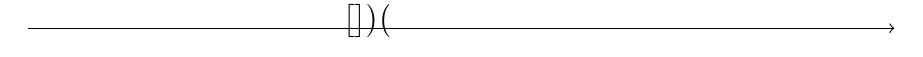
\begin{tikzpicture}
				\draw[->](-4,0)->(7,0);
				\IntervalLR{-4}{-3}
				\IntervalGR{}{}{\big[}{-3}
				\IntervalLR{6}{6.9}
				\IntervalGR{\big]}{6}{}{}
				\IntervalLR{-2}{3}
				\def\skipInterval{0.5cm}
				\IntervalGLF{\big)}{-2}{\big(}{3}
			\end{tikzpicture}
		\end{center}
		Từ hình vẽ, ta có
		Khi đó: $M\cap N= [-3;-2)\cup (3;6]$.}
\end{ex}


\begin{ex}%[Phan Quốc Trí, Bai Giảng T10(2022)]%%[Trần Ngọc Minh]%[301-320-Huỳnh Thanh Tiến]%[0D1B4-1]
	Tập hợp $(1;2)\cap\mathbb{N}$ là tập hợp nào sau đây?
	\choice
	{$\{1;2\}$}
	{$\{1\}$}
	{\True $\varnothing$}
	{$\{2\}$}
	\loigiai{
		Ta có $\mathbb{N}=\{0,1,2,\ldots\}$.
		Do đó 	$(1;2)\cap\mathbb{N}=\varnothing$.
	}
\end{ex}	
\begin{ex}%[Phan Quốc Trí, Bai Giảng T10(2022)]%[0D1B4-1]
	Cho $A=(-5;1]$, $B=[3;+\infty)$, $C=(-\infty;-2)$. Khẳng định nào sau đây đúng?
	\choice
	{$A\cap C=[-5;-2]$}
	{$A\cup B=(-5;+\infty)$}
	{$B\cup C=(-\infty;+\infty)$}
	{$\True B\cap C= \varnothing$}
	\loigiai{
		\begin{center}
			\begin{tikzpicture}
				\draw[->](-1,0)->(5,0);
				\IntervalLR{-1}{3}
				\def\skipInterval{0.5cm}
				\IntervalGRF{}{}{\big[}{3}
				\IntervalLR{4}{4.8}
				\def\skipInterval{0.5cm}
			\end{tikzpicture}\\
			\begin{tikzpicture}
				\draw[->](-1,0)->(5,0);
				\IntervalLR{-1}{1/2}
				\def\skipInterval{0.5cm}
				\IntervalLR{2}{4.9}
				\def\skipInterval{0.5cm}
				\IntervalGRF{\big)}{-2}{}{}
			\end{tikzpicture}
		\end{center}
		Từ biểu diễn tập nghiệm của $B$ và $C$ ta thấy $B\cap C= \varnothing$.
	}
\end{ex}
\begin{ex}%[Phan Quốc Trí, Bai Giảng T10(2022)]%%[0-HK2-2021, Trường THPT Trần Phú, Hải Phòng, năm học 2017 - 2018]%[Trần Quang Thạnh]%[0D1Y4-2]
	Cho tập hợp $A=[-2;3]$ và $B=(-2;5]$. Khi đó $A\setminus B$ là
	\choice
	{$[-2;5] $}
	{$(-2;-1) $}
	{$(3;5) $}
	{\True $\left\{-2\right\} $}
	\loigiai{
		Ta có $A\setminus B=\left\{-2\right\}$.
	}
\end{ex}
\begin{ex}%[Phan Quốc Trí, Bai Giảng T10(2022)]%[0D1B4-2]
	Cho các tập $A=\left\{x\in\mathbb{R}\mid x\ge -1\right\}$; $B=\left\{x\in\mathbb{R}\mid x<3\right\}$. Tập hợp $\mathbb{R}\setminus\left(A\cap B\right)$ là
	\choice
	{$[-1;3)$}
	{$(-\infty;-1]\cup(3;+\infty)$}
	{\True $(-\infty;-1)\cup[3;+\infty)$}
	{$(-1;3]$}
	\loigiai{
		Ta có $A\cap B=[-1;3)$, suy ra $\mathbb{R}\setminus\left(A\cap B\right)=(-\infty;-1)\cup[3;+\infty)$.
	}
\end{ex}
\begin{ex}%[Phan Quốc Trí, Bai Giảng T10(2022)]%[0D1B2-2]
	Tìm tất cả các giá trị của $m$ để đoạn $[m;m+3]$ là tập con của nửa khoảng $(-2;9]$.
	\choice
	{$-2\le m\le 6$}
	{$-2\le m<6$}
	{\True $-2<m\le 6$}
	{$-2<m<6$}
	\loigiai{
		Đoạn $[m;m+3]$ là tập con của nửa khoảng $(-2;9]$ khi và chỉ khi $\heva{& -2<m \\& m+3\le 9}\Leftrightarrow \heva{& -2<m \\& m\le 6}\Leftrightarrow -2<m\le 6.$
	}
\end{ex}



\noindent\textbf{II. PHẦN TỰ LUẬN}
\begin{bt}%[Phan Quốc Trí, Bai Giảng T10(2022)]%[0D1B4-1] 
	Cho $A=\left \{x \in \mathbb{R} \Big|  x \geq 3\right \} ; B=(-2 ; 7]$.  Tìm các tập hợp $A \cap B, A \cup B$.
	\loigiai{
		Ta có $A=\left \{x \in \mathbb{R} \Big|  x \geq 3\right \} = [3;+\infty )$. \\
		$A \cap B =[3;+\infty ) \cap (-2 ; 7] =    [3;7 ]$. \\
		$A \cup B = [3;+\infty ) \cup (-2 ; 7] = (-2;+\infty)$. 
	}
\end{bt}
\begin{bt}%[Phan Quốc Trí, Bai Giảng T10(2022)]%[0D1B3-2]
	Cho hai tập hợp $A=\left\{ 0;2 \right\}$ và $B=\left\{ 0;1;2;3;4 \right\}$. Tìm tất cả các tập hợp $X$ thỏa mãn $A\cup X=B$.
	\loigiai { 
		Vì $A\cup X=B$ nên $X$ chắc chắn có chứa các phần tử $1;3;4$\\
		Các tập $X$ có thể là $\left\{ 1;3;4 \right\},\,\left\{ 1;3;4;0 \right\},\,\left\{ 1;3;4;2 \right\},\,\left\{ 1;3;4;0;2 \right\}$}
\end{bt}
\begin{bt}%[Phan Quốc Trí, Bai Giảng T10(2022)]%[0D1B4-1]
	Cho hai tập hợp $A=(2m-1;m+3)$, $B=(-4;5)$. Tìm $m$ để
	$A\cap B=\varnothing $.
	\loigiai{
		Điều kiện: $2m-1<m+3 \Leftrightarrow m<4$.
		Để $A\cap B=\varnothing $ khi và chỉ khi $\left[
		\begin{aligned}
			&m+3\leqslant -4\\
			&2m-1\geqslant 5
		\end{aligned}\right. \Leftrightarrow \left[
		\begin{aligned}
			&m\leqslant -7\\
			&m\geqslant 3
		\end{aligned}\right. $.\\
		Đối chiếu điều kiện, ta được $m\leqslant -7$ hoặc $3\leqslant m<4$ thỏa yêu cầu bài toán.
	}
\end{bt}
\begin{bt}%[Phan Quốc Trí, Bai Giảng T10(2022)]%[0D1B3-3]
	Lớp 10A có $45$ học sinh, trong đó có $18$ học sinh tham gia cuộc thi vẽ đồ họa trên máy tính, $24$ học sinh tham gia cuộc thi tin học văn phòng cấp trường và $9$ học sinh không tham gia cả hai cuộc thi này. Hỏi lớp 10A có bao nhiêu học sinh tham gia đồng thời cả hai cuộc thi?	
	\loigiai{
		\immini{
			Gọi $A$ là tập hợp các học sinh tham gia cuộc thi vẽ đồ họa trên máy tính. Suy ra $n(A)= 18$.\\
			$B$ là tập hợp các học sinh tham gia  cuộc thi tin học văn phòng cấp trường. Suy ra $n(B)= 24$.\\
			Ta có $A \cap B$ là tập hợp các học sinh tham gia đồng thời cả hai cuộc thi.\\
			$A \cup B$ là tập hợp các học sinh tham gia cuộc thi vẽ đồ họa trên máy tính hoặc tham gia  cuộc thi tin học văn phòng cấp trường. 
		}{
			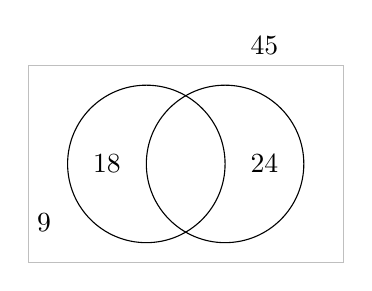
\begin{tikzpicture}
				\draw[] (0,0) circle ( 1.0cm);
				\draw (1.0,0) circle ( 1.0 cm);
				\draw (-0.5,0) node {$18$};
				\draw (1.5,0) node {$24$};
				\draw (-1.3,-0.75) node {$9$};
				\draw (1.5,1.5) node {$45$};
				\node[rectangle,
				draw = lightgray,
				minimum width = 4cm, 
				minimum height = 2.5cm] (r) at (0.5,0) {};
			\end{tikzpicture}
		}
		$$n \left(A \cup B \right)= 45-9=36.$$	
		$$n \left( A \cap B \right) = n(A)+ n(B)-n(A \cup B)=18+24-36= 6.$$
		Vậy có $6$  học sinh tham gia đồng thời cả hai cuộc thi.
	}
\end{bt}

\Closesolutionfile{ans}

\newpage
\begin{indapan}{10}
	{ans/ans-KT-102}
\end{indapan}




\section*{Đề kiểm tra Chương 1}
\subsection*{Đề số 3}
\setcounter{ex}{0}\setcounter{bt}{0}
\Opensolutionfile{ans}[ans/ans-KT-103]
\noindent\textbf{I. PHẦN TRẮC NGHIỆM}
%[Thi thử, Sở GD và ĐT - Điện Biên, 2018]%[Dương BùiĐức, 12EX10]%[2D2Y3-2]
\begin{ex}%[Phan Quốc Trí, Bai Giảng T10(2022)]%[0D1Y1-1]
	Câu nào trong các câu sau \textbf{không phải} là mệnh đề?
	\choice
	{\True $\pi$ có phải là một số vô tỷ không?}
	{$2+2=5$}
	{$\sqrt{2}$ là một số hữu tỷ}
	{$\dfrac{4}{2}=2$}
	\loigiai{
		\lq\lq $\pi$ có phải là một số vô tỷ không?\rq\rq\, là câu hỏi, nên không phải là mệnh đề.
	}
\end{ex}
\begin{ex}%[Phan Quốc Trí, Bai Giảng T10(2022)]%[0D1Y1-1]
	Phát biểu nào sau đây là một mệnh đề?
	\choice
	{Mùa thu Hà Nội đep quá!}
	{\True Hà Nội là thủ đô của Việt Nam}
	{Bạn có đi học không?}
	{Đề thi môn Toán khó quá!}
	\loigiai{
		Hà Nội là thủ đô của Việt Nam là một khẳng định đúng.
	}
\end{ex}
\begin{ex}%[Phan Quốc Trí, Bai Giảng T10(2022)]%[0D1Y1-2]
	Trong các mệnh đề sau, mệnh đề nào \textbf{sai}?
	\choice
	{$-2 \in \mathbb{Q}$}
	{$\sqrt{2} \in \mathbb{R}$}
	{\True $\dfrac{1}{2} \in \mathbb{Z}$}
	{$2 \in \mathbb{N}$}
	\loigiai{
		Mệnh đề sai là  $\dfrac{1}{2} \in \mathbb{Z}$.
	}
\end{ex}
\begin{ex}%[Phan Quốc Trí, Bai Giảng T10(2022)]%[0D1Y1-2]
	Cho mệnh đề chứa biến $P(n) \colon$ "$n^2-1$ chia hết cho $4$" với $n$ là số nguyên. Khẳng định nào sau đây đúng?
	\choice
	{$P(5)$ đúng và $P(2)$ đúng}
	{\True $P(5)$ đúng và $P(2)$ sai}
	{$P(5)$ sai và $P(2)$ sai}
	{$P(5)$ sai và $P(2)$ đúng}
	\loigiai{
		Ta có:\\
		$P(5) \colon$ "$5^2-1$ chia hết cho $4$" tức là "$24$ chia hết cho $4$", nên $P(5)$ đúng.\\
		$P(2) \colon$ "$2^2-1$ chia hết cho $4$" tức là "$3$ chia hết cho $4$", nên $P(2)$ sai.\\
		Vậy $P(5)$ đúng và $P(2)$ đúng.}
\end{ex}
\begin{ex}%[Phan Quốc Trí, Bai Giảng T10(2022)]%[0D1Y1-3]
	Phủ định của mệnh đề: ``$\pi$ là số vô tỷ'' là
	\choice
	{$\pi$ là số nguyên}
	{$\pi$ là số dương}
	{$\pi$ là số thực}
	{\True $\pi$ không phải là số vô tỷ}	
	\loigiai{Mệnh đề phủ định là ``$\pi$ không phải là số vô tỷ''.}
\end{ex}
\begin{ex}%[Phan Quốc Trí, Bai Giảng T10(2022)]%[0D1Y1-3]
	Mệnh đề phủ định của mệnh đề \lq \lq $\exists x\in \mathbb{N}\colon x^2-4=0$\rq \rq \ là
	\choice
	{\lq \lq $\forall x\in \mathbb{N}\colon x^2-4=0$\rq \rq }
	{\lq \lq $\forall x\in \mathbb{N}\colon x^2-4>0$\rq \rq }
	{\lq \lq $\exists x\in \mathbb{N}\colon x^2-4\ne 0$\rq \rq }
	{\True \lq \lq $\forall x\in \mathbb{N}\colon x^2-4\ne 0$\rq \rq}
	\loigiai{
		Ta có mệnh đề phủ định của mệnh đề \lq\lq $\exists x \in X, P(x)$\rq\rq\ là \lq\lq $\forall x \in X, \overline{P(x)}$\rq\rq.\\
		Nên mệnh đề phủ định của mệnh đề \lq \lq $\exists x\in \mathbb{N}\colon x^2-4=0$\rq \rq \ là \lq \lq $\forall x\in \mathbb{N}\colon x^2-4\ne 0$\rq \rq.
	}
\end{ex}
\begin{ex}%[Phan Quốc Trí, Bai Giảng T10(2022)]%[0D1Y1-4]
	Cho mệnh đề $P\colon$ ``$b^2\ge 4ac$'', mệnh đề $Q\colon$ ``Phương trình $ax^2 +bx+c=0$ vô nghiệm'' (với $a,b,c$ là số thực và $a\ne 0$). Phát biểu mệnh đề ``$P$ kéo theo $Q$'' là
	\choice
	{Nếu Phương trình $ax^2 +bx+c=0$ vô nghiệm thì $b^2\ge 4ac$ (với $a,b,c$ là số thực và $a\ne 0$)}
	{\True Nếu $b^2\ge 4ac$ thì phương trình $ax^2 +bx+c=0$ vô nghiệm (với $a,b,c$ là số thực và $a\ne 0$) }
	{$b^2\ge 4ac$ là điều kiện cần và đủ để phương trình $ax^2 +bx+c=0$ vô nghiệm (với $a,b,c$ là số thực và $a\ne 0$)}
	{$b^2\ge 4ac$ khi và chỉ khi phương trình $ax^2 +bx+c=0$ vô nghiệm (với $a,b,c$ là số thực và $a\ne 0$)}
	\loigiai{
		Mệnh đề ``$P$ kéo theo $Q$'' là ``Nếu $b^2\ge 4ac$ thì phương trình $ax^2 +bx+c=0$ vô nghiệm (với $a,b,c$ là số thực và $a\ne 0$)''.
	}
\end{ex}
\begin{ex}%[Phan Quốc Trí, Bai Giảng T10(2022)]%[0D1Y1-4]
	Cho mệnh đề $P$: \lq\lq Nếu tam giác $ABC$ có hai góc bằng $60^{\circ}$ thì đó là tam giác$ABC$ đều\rq\rq. Mệnh đề nào sau đây là mệnh đề đảo của $P$?
	\choice
	{Tam giác $ABC$ có hai góc bằng $60^{\circ}$ thì đó là tam giác$ABC$ đều}
	{\True Nếu tam giác $ABC$ đều thì tam giác đó có hai góc bằng $60^{\circ}$}
	{Tam giác $ABC$ đều khi và chỉ khi tam giác đó có hai góc bằng $60^{\circ}$}
	{Tam giác$ABC$ đều nếu nó có hai góc bằng $60^{\circ}$}
	\loigiai{
		Mệnh đề đảo là \lq \lq Nếu tam giác $ABC$ đều thì tam giác đó có hai góc bằng $60^{\circ}$.\rq \rq		
	}
\end{ex}
\begin{ex}%[Phan Quốc Trí, Bai Giảng T10(2022)]%[0D1Y1-5]
	Mệnh đề "Có ít nhất một số tự nhiên khác 0" mô tả mệnh đề nào dưới đây?
	\choice{"$\forall n\in\mathbb{N}: n\neq 0$"}
	{"$\exists x\in\mathbb{N}:x=0$"}
	{"$\exists x\in\mathbb{Z}: x\neq 0$"}
	{\True "$\exists x\in\mathbb{N}:x\neq 0$"}
	\loigiai{
		Mệnh đề được viết lại là: "$\exists x\in\mathbb{N}:x\neq 0$".}
\end{ex}
\begin{ex}%[Phan Quốc Trí, Bai Giảng T10(2022)]%[0D1Y1-5]
	Mệnh đề nào sau đây đúng?
	\choice{$\forall n\in\mathbb{N}: n > 0$}
	{\True $\exists m\in\mathbb{Z}:2m=m$}
	{$\forall x\in\mathbb{R}:x^2> 0$}
	{$\exists k\in\mathbb{Q}:k^2=2$}
	\loigiai{
		Mệnh đề $\forall n\in\mathbb{N}: n > 0$ là mệnh đề sai, ví dụ $n=0$.\\
		Mệnh đề $\exists m\in\mathbb{Z}:2m=m$ là mệnh đề đúng, vì tồn tại $m=0$ thỏa mãn.\\
		Mệnh đề $\forall x\in\mathbb{R}:x^2> 0$ là mệnh đề sai, ví dụ $x=0$.\\
		Mệnh đề $\exists k\in\mathbb{Q}:k^2=2$ là mệnh đề sai.}
\end{ex}
\begin{ex}%[Phan Quốc Trí, Bai Giảng T10(2022)]%[0D1Y2-1]
	Hãy liệt kê các phần tử của tập $X=\left\{ x \in \mathbb{Q}| (x^2-x-6)(x^2-5)=0 \right\}$.
	\choice
	{$X=\left\{ \sqrt{5};3 \right\}$}
	{\True $X=\left\{ -2;3 \right\}$}
	{$X=\left\{ -\sqrt{5};-2;\sqrt{5}; 3 \right\}$}
	{$X=\left\{ -\sqrt{5};\sqrt{5}  \right\}$}
	\loigiai{
		Ta có 
		\begin{itemize}
			\item $x^2-x-6 = 0 \Leftrightarrow \hoac{&x=3 \in \mathbb{Q} \\&x=-2 \in \mathbb{Q}. }$
			\item $x^2-5 =0 \Leftrightarrow \hoac{&x= \sqrt{5} \notin \mathbb{Q} \\& x= - \sqrt{5} \notin \mathbb{Q}.}$
		\end{itemize}
		Do đó $X=\left\{ -2;3 \right\}$.
	}
\end{ex}
\begin{ex}%[Phan Quốc Trí, Bai Giảng T10(2022)]%[0D1Y2-1]
	Hãy liệt kê các phần tử của tập hợp $X=\left\{x \in \mathbb{N} \ |  \ x \leq 3\right\}$
	\choice
	{$X=\left[0;3\right]$}
	{\True $X=\left\{0;1;2;3\right\}$}
	{$X=\left\{1;2;3\right\}$}
	{$X=\left\{0  \longrightarrow 3\right\}$}
	\loigiai{ 
		Liệt kê các phần tử của tập hợp $X=\left\{x \in \mathbb{N} \ | \ x \leq 3\right\}=\left\{0;1;2;3\right\}$.
	}
\end{ex}

\begin{ex}%[Phan Quốc Trí, Bai Giảng T10(2022)]%[0D1Y2-1]
	Cho tập hợp $A=\{x\in \mathbb{R}|x^2-2x+5=0\}$. Mệnh đề nào sau đây đúng?
	\choice
	{\True $A=\varnothing$}
	{$A=0$}
	{$A=\{-1\}$}
	{$A=\{0\}$}
	\loigiai{
		Vì phương trình $x^2-2x+5=0$ vô ngiệm nên $A=\varnothing$.	
	}	
\end{ex}
\begin{ex}%[Phan Quốc Trí, Bai Giảng T10(2022)]%[0D1Y2-2]
	Cho tập hợp $A=\{a;b;c;d\}$. Số tập hợp con của $A$ có hai phần tử là
	\choice
	{\True $6$}
	{$7$}
	{$8$}
	{$5$}
	\loigiai{
		Sô tập con có hai phần tử của tập $A$ là $6$ đó là các tập $\{a;b\}$, $\{a;c\}$, $\{a;d\}$, $\{b;c\}$, $\{b;d\}$, $\{c;d\}$.}
\end{ex}
\begin{ex}%[Phan Quốc Trí, Bai Giảng T10(2022)]%[0D1Y2-2]
	Có bao nhiêu tập $A$ để $\{m; n\} \subset A \subset \{m; n; x; y\}$? 
	\choice
	{$2$}
	{$3$}
	{$1$}
	{\True $4$}
	\loigiai{
		Các tập $A$ thỏa mãn là $\{m; n\}$, $\{m; n; x\}$, $\{m; n; y\}$ và $\{m; n; x; y\}$. 
	}
\end{ex}
\begin{ex}%[Phan Quốc Trí, Bai Giảng T10(2022)]%[0D1B4-1]
	Cho tập hợp $X = \left\{x \in \mathbb{R}\big|- 2\le x \le 5\right\}$. Khẳng định nào sau đây đúng?
	\choice{$X = \left(-2;5\right)$}
	{$X = \left\{-2;5\right\}$}
	{$X = \left[-2;5\right)$}
	{\True $X = \left[-2;5\right]$}
	\loigiai{
		$\left\{x \in \mathbb{R}\big|- 2\le x \le 5\right\}= \left[-2;5\right]$.
	}
\end{ex}
\begin{ex}%[Phan Quốc Trí, Bai Giảng T10(2022)]%[0D1B2-2]
	Cho tập hợp $A = \left\{x \in \mathbb{N}\big| x^2 + 3x  = 0\right\}$. Khẳng định nào sau đây đúng?
	\choice
	{$A = \left\{-3;0\right\}$}
	{$A =\varnothing$}
	{$A = \left\{\varnothing\right\}$}
	{\True $ A = \left\{0\right\}$}
	\loigiai{
		Phương trình $x^2+3x=0$ có hai nghiệm $x_1=-3$, $x_2=0$. Tuy nhiên chỉ $x_1=0 \in \mathbb{N}$. Vậy $A=\left\{0\right\} $.
	}
\end{ex}
\begin{ex}%[Phan Quốc Trí, Bai Giảng T10(2022)]%[0D1B2-2]
	Gọi $A$ là tập hợp tất cả các tam giác cân và $B$ là tập hợp tất cả các tam giác đều. Trong các kết luận sau, kết luận nào đúng?
	\choice
	{$A \subset B$}
	{\True $B \subset A$}
	{$A=B$}
	{$A \cap B=\varnothing$}
	\loigiai{
		Ta có tam giác đều là một tam giác cân và có một góc $60^{\circ}$ nên $B \subset A$.
	}
\end{ex}

\begin{ex}%[Phan Quốc Trí, Bai Giảng T10(2022)]%[0D1B2-2]
	Cho $\mathbb{N}$, $\mathbb{Z}$, $\mathbb{Q}$, $\mathbb{R}$ là các tập hợp số. Mệnh đề nào sau đây \textbf{sai}?
	\choice
	{$\mathbb{Q} \subset \mathbb{R}$}
	{$\mathbb{N} \subset \mathbb{Z} \subset \mathbb{Q} \subset \mathbb{R}$}
	{$\mathbb{N} \subset \mathbb{Z} \subset \mathbb{Q}$}
	{\True $\mathbb{R} \subset \mathbb{Z}$}
	\loigiai{
		Theo mối quan hệ giữa các tập hợp số, ta có $\mathbb{N} \subset \mathbb{Z} \subset \mathbb{Q} \subset \mathbb{R}$.
	}
\end{ex}
\begin{ex}%[Phan Quốc Trí, Bai Giảng T10(2022)]%[0D1Y3-1]
	Cho tập hợp $M=\{1;2;3\}$ và $N=\{1;a;b\}$. Tìm $M\cup N$.
	\choice
	{\True $M\cup N=\{1;2;3;a;b\}$}
	{$M\cup N=\{2;3;a;b\}$}
	{$M\cup N=\{1\}$}
	{$M\cup N=\{2;3\}$}
	\loigiai{
		$M\cup N=\{1;2;3;a;b\}$.
	}
\end{ex}
\begin{ex}%[Phan Quốc Trí, Bai Giảng T10(2022)]%[0D1Y3-1]
	Cho hai tập hợp $A=\{a;c;d;e\}$ và $B=\{c;d;f;1;2\}$. Khi đó $A\cap B$ là	
	\choice
	{$\{1;2;f\}$}
	{$\{c;d;a;e;f;1;2\}$}
	{\True $\{c;d;\}$}
	{$\{a;e\}$}
	\loigiai{
		Ta có $A\cap B=\{c;d\}$.	
	}
\end{ex}
\begin{ex}%[Phan Quốc Trí, Bai Giảng T10(2022)]%[0D1Y3-2]
	Cho hai tập hợp $A= \left\{0, 1, 2,3,4,5,7\right\}$  và $B= \left\{2,3,4,5,6\right\}$. Tập hợp $A \setminus B$ bằng 
	\choice
	{$ \left\{0,1,2,7\right\}$}
	{$\left\{0,7\right\}$}
	{\True  $\left\{0,1,7\right\}$}
	{$\left\{0,1,6,7\right\}$}
	\loigiai{
		Ta có \[A \setminus B=\left\{0, 1, 7\right\}.\]
	}
\end{ex}

\begin{ex}%[Phan Quốc Trí, Bai Giảng T10(2022)]%[0D1Y3-2]
	Cho hai tập hợp $M=\{0;2;4;6;8;10\}$ và $N=\{0;1;2;3;4;5;6;7;8;9;10\}$. Hãy tìm phần bù của $M$ trong tập hợp $N$.
	\choice
	{$C_NM=N $}
	{$C_NM=M $}
	{\True $C_NM=\{1;3;5;7;9\} $}
	{$C_NM=\{0;2;6;8\} $}
	\loigiai{
		Vì $C_NM$ là tập hợp tất cả các phần tử của $N$ nhưng không là phần tử của $M$, do đó $C_NM= \{1;3;5;7;9\} $.
	}
\end{ex}
\begin{ex}%[Phan Quốc Trí, Bai Giảng T10(2022)]%[0D1B4-1]
	Cho $A=(-\infty;5]$ và $B=(0;+\infty)$. Tập hợp $A\cap B$ là
	\choice
	{\True $(0;5]$}
	{$[0;5)$}
	{$(0;5)$}
	{$(-\infty;+\infty)$}
	\loigiai
	{
		\begin{center}
			\begin{tikzpicture}[scale=1, font=\footnotesize, >=stealth]
				\draw[->] (0,0)--(9,0);
				\draw (3,0) node{$\Big($} + (90:.5) node{$0$} (6,0) node{$\Big]$} + (90:.5) node{$5$};
				\fill[pattern=north east lines] (0,-3pt) rectangle (3,3pt) (6,-3pt) rectangle (9,3pt);
				\begin{scope}[on background layer]\path[white]node{MDD-138};\end{scope}
			\end{tikzpicture}
		\end{center}
		Ta có $A\cap B = (-\infty;5]\cap (0;+\infty) = (0;5]$.
	}
\end{ex}
\begin{ex}%[Phan Quốc Trí, Bai Giảng T10(2022)]%[0D1B4-1]
	Cho tập hợp $A=[-2;5)$ và $B=[0;+\infty)$. Tìm $A\cup B$.
	\choice
	{$A\cup B=[0;5)$}
	{$A\cup B=[-2;0)$}
	{\True $A\cup B=[-2;+\infty)$}
	{$A\cup B[5;+\infty)$}
	\loigiai{
		Ta có 	$A\cup B=[-2;+\infty)$.
	}
\end{ex}

\begin{ex}%[Phan Quốc Trí, Bai Giảng T10(2022)]%[0D1B4-2]
	Tập hợp $\left( -2;3 \right)\setminus \left[1;6 \right]$ bằng tập hợp nào sau đây?
	\choice
	{$\left(-2;1\right]$}
	{$\left(-3;-2\right)$}
	{$\left(-2;6\right)$}
	{\True $\left(-2;1\right)$}
	\loigiai{Ta có $\left(-2;3\right)\setminus \left[1;6\right]=\left(-2;1\right)$.
	}
\end{ex}

\begin{ex}%[Phan Quốc Trí, Bai Giảng T10(2022)]%[0D1B4-2]
	Cho tập hợp $A=\left[ -2;\,\sqrt{5} \right)$. Tập hợp $C_{\mathbb{R}}A$ bằng
	\choice
	{$\left( -\infty ;\,-2 \right]\cup \left[ \sqrt{5};\,+\infty \right)$}
	{\True $\left( -\infty ;\,-2 \right)\cup \left[ \sqrt{5};\,+\infty \right)$}
	{$\left( -\infty ;\,-2 \right]\cup \left( \sqrt{5};\,+\infty \right)$}
	{$\left( -\infty ;\,-2 \right)\cup \left( \sqrt{5};\,+\infty \right)$}
	\loigiai{
		Ta có $C_{\mathbb{R}}A=\Bbb{R}\setminus A=\left( -\infty ;\,-2 \right)\cup \left[ \sqrt{5};\,+\infty \right).$
	}
\end{ex}
\begin{ex}%[Phan Quốc Trí, Bai Giảng T10(2022)]%[0D1B3-3]
	Một lớp có $40$ học sinh, trong đó có $24$ học sinh giỏi Toán, $18$ học sinh giỏi Văn và $10$ học
	sinh không giỏi môn nào trong hai môn Toán và Văn. Hỏi lớp đó có bao nhiêu học sinh giỏi cả hai môn
	Toán và Văn?
	\choice
	{\True $12$ học sinh}
	{$8$ học sinh}
	{$10$ học sinh}
	{$14$ học sinh}
	\loigiai{
		Số học sinh giỏi ít nhất một trong hai môn Toán và Văn là $40-10=30$.\\
		Do có $24$ học sinh giỏi Toán, $18$ học sinh giỏi Văn nên số học sinh giỏi cả hai môn là
		\[24+18-30=12.\]
	}	
\end{ex}
\begin{ex}%[Phan Quốc Trí, Bai Giảng T10(2022)]%[0D1B3-3]
	Mỗi học sinh lớp 10A phải học ít nhất một trong hai môn ngoại ngữ tiếng Anh hoặc tiếng Nhật. Biết lớp 10A có $51$ bạn học sinh trong đó có $31$ bạn học tiếng Anh và $27$ bạn học tiếng Nhật. Hỏi lớp 10A có bao nhiêu bạn học cả tiếng Anh và tiếng Nhật?
	\choice
	{\True $7$}
	{$9$}
	{$5$}
	{$12$}
	\loigiai{
		Số học sinh học cả tiếng Anh và tiếng Nhật của lớp 10A là $31+27-51=7$ bạn.
	}
\end{ex}
\begin{ex}%[Phan Quốc Trí, Bai Giảng T10(2022)]%[0D1B4-1]
	Cho hai tập hợp $A=(-4;5) \cup (7;9)$ và $B=(2;8)$. Tìm $A\cap B$ ta được
	\choice
	{$A \cap B=(7;8)$}
	{$A \cap B=(2;5)$}
	{\True $A \cap B=(2;5) \cup (7;8)$}
	{$A \cap B=[2;5] \cup [7;8]$}
	\loigiai{
		Ta có $A\cap B = \left[(-4;5) \cup (7;9)\right] \cap (2;8)=\left[(-4;5) \cap (2;8)\right] \cup \left[(7;9) \cap (2;8)\right]=(2;5)\cup (7;8)$.	
	}
\end{ex}

\begin{ex}%[Phan Quốc Trí, Bai Giảng T10(2022)]%[0D1B4-1]
	Cho hai tập $A=(-2; 4] \cap \mathbb{Z}$, $B=[-5; 7] \cap \mathbb{N}^{*}$. Số phần tử của tập hợp $A \cup B$ là
	\choice
	{\True $9$}
	{$13$}
	{$10$}
	{$8$}
	\loigiai{
		$A=(-2; 4] \cap \mathbb{Z}=\{-1;0;1;2;3;4\}$, $B=[-5; 7] \cap \mathbb{N}^{*}=\{1;2;3;4;5;6;7\}$.\\
		Ta có $A \cup B=\{-1;0;1;2;3;4;5;6;7\}$. Vậy tập hợp $A \cup B$ có $9$ phần tử.
	}
\end{ex}
\begin{ex}%[Phan Quốc Trí, Bai Giảng T10(2022)]%[0D1B4-1]
	Cho các tập hợp $A=\left[-2;2\right]$, $B=\left(1;5\right]$ và $ C=\left[0;3\right)$. Khi đó tập $\left(A \setminus B\right)\cap C$ là
	\choice
	{\True $\left[0;1\right]$}
	{$\left\{0;1\right\}$}
	{$\left[0;1\right)$}
	{$\left(0;1\right]$}
	\loigiai{
		Ta có $ A\setminus B=\left[-2;1\right]$$\Rightarrow\left(A\setminus B\right)\cap C=\left[0;1\right]$.
	}
\end{ex}
\begin{ex}%[Phan Quốc Trí, Bai Giảng T10(2022)]%[0D1Y4-2]
	Cho tập hợp $A=(-2;1]$ và $B=[-2;8)$. Khi đó $A\setminus B$ bằng
	\choice
	{$\left\{ 2 \right\}$}
	{$(1;8) $}
	{$\left\{ 8 \right\}$}
	{\True $\varnothing$}
	\loigiai{
		Ta có $A\setminus B=\varnothing$.
	}
\end{ex}
\begin{ex}%[Phan Quốc Trí, Bai Giảng T10(2022)]%[0D1B4-2]
	Cho $A=\left\{x\in \mathbb{R}|x+1\ge 0\right\}$, $B=\left\{x\in \mathbb{R}|4-x\ge 0\right\}$. Khi đó $A\backslash B$ là 
	\choice
	{$\left[-1; 4\right]$}
	{$\left[4;+\infty\right)$}
	{\True $\left(4;+\infty\right)$}
	{$\left(-\infty;-1\right)$}
	\loigiai{
		$A=\left\{x\in \mathbb{R}|x+1\ge 0\right\}=\left[-1;+\infty\right)$; $B=\left\{x\in \mathbb{R}|4-x\ge 0\right\}=\left(-\infty; 4\right]$.\\
		Nên $A\backslash B=\left(4;+\infty\right)$.
	}
\end{ex}
\begin{ex}%[Phan Quốc Trí, Bai Giảng T10(2022)]%[0D1K4-2]
	Cho tập hợp $A=[m;m+1]$, $B=[1;3]$. Tập hợp tất cả các giá trị của $m$ để $A\subset B$ là
	\choice
	{$m\leq 1$ hoặc $m\geq 2$}
	{\True $1\leq m\leq 2$}
	{$1<m<2$}
	{$0\leq m\leq 2$}
	\loigiai{Để $A\subset B$ thì $\heva{&m\geq 1\\&m+1\leq 3}\Leftrightarrow 1\leq m\leq 2$.}
\end{ex}
\noindent\textbf{II. PHẦN TỰ LUẬN}
\begin{bt}%[Phan Quốc Trí, Bai Giảng T10(2022)]%[0D1B4-1] 
	Cho $A=\left \{x \in \mathbb{R} \Big|  -1<x \le 7 \right \} ; B=(-\infty ; 2]$.  Tìm các tập hợp $A \cap B, A \cup B$.
	\loigiai{
		Ta có $A = (-1;7]$, $A \cap B = (-1;2]$ và 
		$A \cup B = (-\infty ; 7] $. 
	}
\end{bt}
\begin{bt}%[Phan Quốc Trí, Bai Giảng T10(2022)]%[0D1B3-2]
	Cho hai tập hợp $A=\left\{ a;b \right\}$ và $B=\left\{ a;b;c;2;3;4 \right\}$. Tìm tất cả các tập hợp $X$ thỏa mãn $A\cup X=B$.
	\loigiai { 
		Vì $A\cup X=B$ nên $X$ chắc chắn có chứa các phần tử $c;2;3;4$\\
		Các tập $X$ có thể là $\left\{ c;2;3;4 \right\},\,\left\{ c;2;3;4;a \right\},\,\left\{ c;2;3;4;b \right\},\,\left\{ c;2;3;4; a;b \right\}$.
	}
\end{bt}
\begin{bt}%[Phan Quốc Trí, Bai Giảng T10(2022)]%[0D1K4-1]
	Cho hai tập khác rỗng $A=(m-1;4]$; $B=(-2;2m+2)$, $m\in\mathbb{R}$. Tìm tất cả các giá trị của $m$ để $A\cap B\neq\varnothing$.
	\loigiai{
		Điều kiện: $\heva{&m-1<4\\&2m+2>-2} \Leftrightarrow -2<m<5$.\\
		Ta có	$A\cap B \ne \varnothing \Leftrightarrow 2m+2> m-1\Leftrightarrow m>-3$.\\
		Kết hợp với điều kiện ta có  $A\cap B \ne \varnothing\Leftrightarrow -3 < m < 5$.
	}
\end{bt}

\begin{bt}%[Phan Quốc Trí, Bai Giảng T10(2022)]%[0D1B3-3]
	Trong số $40$ học sinh của lớp 10A có $12$ bạn được xếp loại học lực giỏi, $19$ bạn được xếp loại hạnh kiểm tốt, trong đó có $8$ bạn vừa có học lực giỏi, vừa có hạnh kiểm tốt. Để được khen thưởng thì bạn đó phải có học lực giỏi hoặc có hạnh kiểm tốt. Hỏi có bao nhiêu bạn \textbf{không} được khen thưởng?
	\loigiai{
		Gọi $A$ là tập hợp các học sinh được xếp loại học lực giỏi, $B$ là tập hợp các học sinh được xếp loại hạnh kiểm tốt.\\
		Ta có 
		\begin{itemize}
			\item $A\cup B$ là tập hợp các học sinh được xếp loại học lực giỏi hoặc hạnh kiểm tốt.
			\item $A\cap B$ là tập hợp các học sinh được xếp loại học lực giỏi và hạnh kiểm tốt.
			\item Theo đề  $$n(A)=12, n(B)=19, n(A\cap B)=8.$$
			\item Do đó $$n(A\cup B=n(A)+n(B)-n(A \cap B))=23.$$
		\end{itemize}
		Vậy lớp 10A có $23$ học sinh được khen thưởng và $17$ học sinh \textbf{không} được khen thưởng.}
\end{bt}

\Closesolutionfile{ans}

\newpage
\begin{indapan}{10}
	{ans/ans-KT-103}
\end{indapan}